\documentclass[11pt]{article}
\usepackage[layoutsize={8.5in,11in},margin=1in]{geometry}\usepackage{graphicx}\usepackage{amsmath}\usepackage{amssymb}\usepackage{amsthm}\usepackage{mathrsfs}\usepackage{bm}\usepackage{pifont}\usepackage[dvipsnames,svgnames,x11names]{xcolor}\usepackage{setspace}\usepackage{pdfcomment}\usepackage{indentfirst}\usepackage{float}\usepackage{braket}\usepackage{enumerate}\usepackage{cleveref}\usepackage{tikz}\tikzset{vertex/.style={circle,draw=black,thick}}\tikzset{arrow/.style={-Stealth,thick}}\usetikzlibrary{decorations.pathmorphing,decorations.text,shapes.geometric,3d,positioning,arrows.meta}

\begin{document}

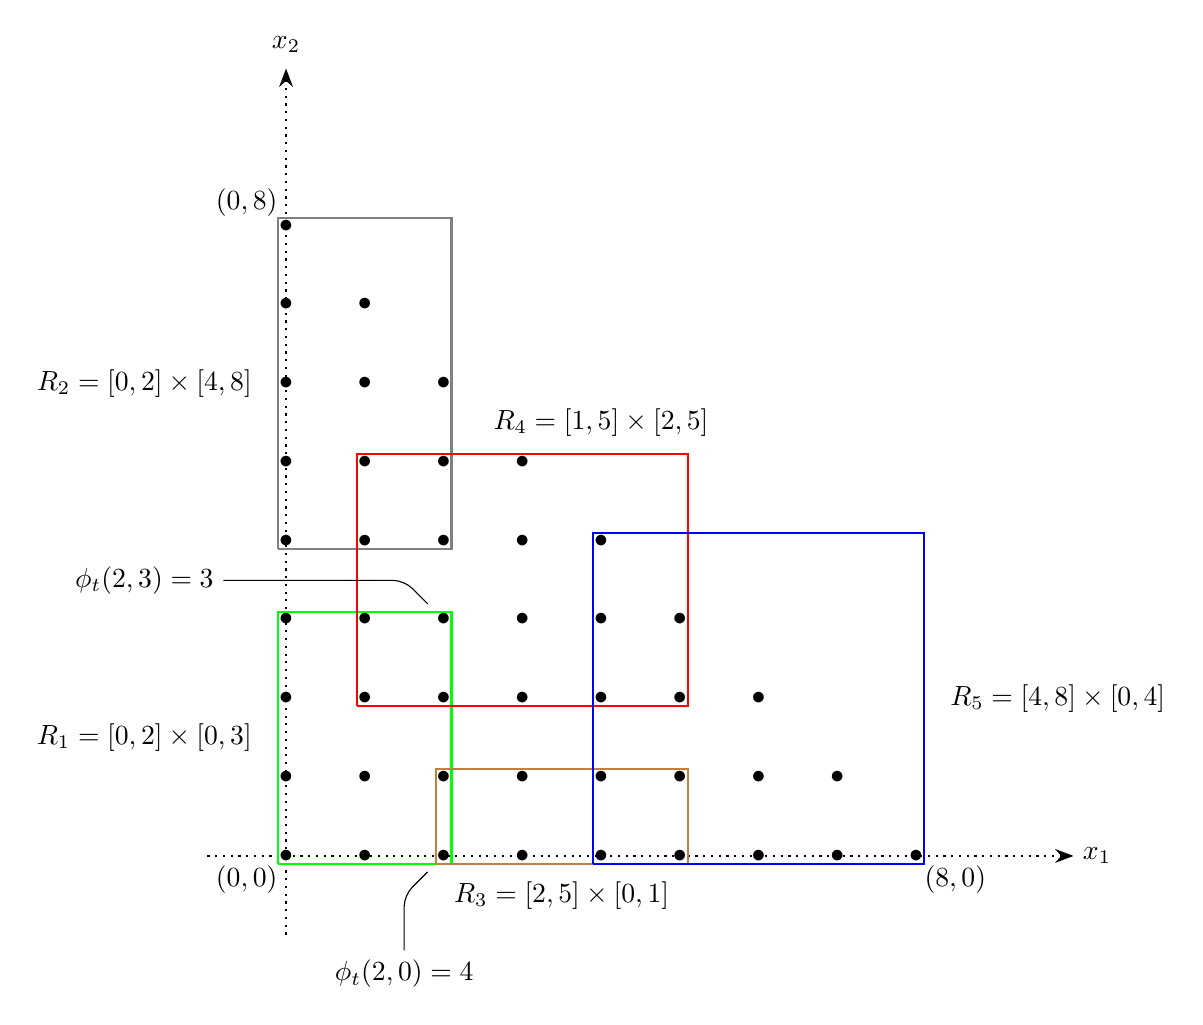
\begin{tikzpicture}
	\foreach \i in {0,...,8} {
		\foreach \j in {0,...,\numexpr8-\i\relax} {
			\node (\i--\j) at (\i,\j) {$\bullet$};
		}
	}
	\draw[arrow,dotted] (-1,0)--(10,0);
	\draw[arrow,dotted] (0,-1)--(0,10);
	\node at (10.3,0) {$x_1$};
	\node at (0,10.3) {$x_2$};
	\node at (-0.5,-0.3) {$(0,0)$};
	\node at (-0.5,8.3) {$(0,8)$};
	\node at (8.5,-0.3) {$(8,0)$};
	\newcommand{\rect}[5]{\draw[thick,#1] (#2-0.1,#4-0.1)--(#3+0.1,#4-0.1)--(#3+0.1,#5+0.1)--(#2-0.1,#5+0.1)--(#2-0.1,#4-0.1)}
	\rect{green}0203;
	\node at (-1.8,1.5) {$R_1=[0,2]\times[0,3]$};
	\rect{gray}0248;
	\node at (-1.8,6) {$R_2=[0,2]\times[4,8]$};
	\rect{brown}2501;
	\node at (3.5,-0.5) {$R_3=[2,5]\times[0,1]$};
	\rect{red}1525;
	\node at (4,5.5) {$R_4=[1,5]\times[2,5]$};
	\rect{blue}4804;
	\node at (9.8,2) {$R_5=[4,8]\times[0,4]$};
	\node(Ex1) at (1.5,-1.5) {$\phi_t(2,0)=4$};
	\draw[rounded corners] (Ex1)--(1.5,-0.5)--(2--0);
	\node(Ex2) at (-1.8,3.5) {$\phi_t(2,3)=3$};
	\draw[rounded corners] (Ex2)--(1.5,3.5)--(2--3);
\end{tikzpicture}

\end{document}